% Chapter IMPLEMENTACJA

\chapter{Realizacja} % Chapter title
Rozdział ten przedstawia opis szczegółowy koncepcji przedstawionych w rozdziale 3.
\section{Oprogramowanie}
\subsection{Narzędzia i środowisko pracy}
Jako środowisko robocze wykorzystano system Ubuntu 14.04. Do stworzenia aplikacji użyte zostało środowisko programistyczne Eclipse Kepler. Dzięki wielu wtyczkom dostępnym do tego IDE (ang. Integrated Development Environment), możliwa była min. wygodna współpraca z systemem kontroli wersji GIT. System kontroli wersji pozwolił na bezpieczne rozwijanie projektu, wraz z możliwością śledzenia istotnych zmian.

\begin{description}
\item Aby zapewnić poprawne działanie zarówno serwera HTTP, jak i kamery niezbędne są:
	\begin{itemize}[noitemsep]
	\item Sterownik UV4L - User-space Video for Linux autorstwa Luci Risolii. Jest to pakiet modułów przeznaczony dla rzeczywistych i wirtualnych urządzeń video  działający w przestrzeni użytkownika, kompatybilny z oficjalnym frameworkiem Video4Linux2 (Video for Linux 2). Moduł uv4l ładuje z poziomu linii komend wybrany sterownik i tworzy węzeł urządzenia video w katalogu /dev głównego systemu plików. Taki interfejs komunikacji z urządzeniem jest popularny w bibliotekach wykorzystujących strumienie video.\\
\begin{description}
\item Do niektórych cech pakietu należą : \\
\begin{itemize}[noitemsep]
\item Kompatybilność z Video4Linux 2 API
\item Dzięki pracy modułów w przestrzeni użytkownika, system (jądro) nie jest narażone na niestabilność
\item Możliwość dodania kilku urządzeń (każde z nich obsługiwane przez oddzielny proces)
\item Nie wymaga zewnętrznych bibliotek i pakietów
\end{itemize}
\end{description}
\begin{description}
\item W pakiecie dostępne są min. moduły:
\begin{itemize}[noitemsep]
\item UV4L core module - główny moduł 
\item Raspicam - moduł dla dedykowanej kamery Raspicam (sensor OV5647)
\item HTTP Streaming Server - sterownik przeznaczony do streamingu video z wykorzystaniem protokołu HTTP\\ 

\end{itemize}
\end{description}
W pracy wykorzystywane są dwa pierwsze, jednak wykorzystanie ostatniego z wymienionych daje możliwości rozszerzenia funkcjonalności kamery.\\
Obsługa pakietu z poziomu linii komend jest następująca:\\

uv4l $--$driver [moduł] $--$video\_nr [numer] $--$encoding [kodowanie] $--$width [szerokość] $--$height [wysokość] \\

Przykładowe wywołanie sterownika:\\
\begin{lstlisting}[caption = {Składnia wywołania sterownika UV4L}, label=UV4L, language=BASH]
 uv4l --driver raspicam --video_nr 0 --encoding yuv420 --width 640
  --height 480
\end{lstlisting}
Uruchomi moduł raspicam, który zarejestruje urządzenie pod węzłem /dev/video0 z kodowaniem strumienia YUV420 i rozdzielczością 640x480.\\
	\item Serwer HTTP Apache 2
Do pracy z przygotowanymi skryptami PHP i jQuery serwer został odpowiednio skonfigurowany. 
		\end{itemize}
\end{description}


\subsection{Algorytm}
Działanie aplikacji opiera się o główny algorytm, który zaprezentowany jest na rysunku\ref{fig:algorytm}. Poniżej znajduje się jego opis :\\
\begin{enumerate}
\item Po starcie programu następuje jego konfiguracja - tworzony jest moduł\textbf{ Controllera} oraz moduły robocze. W zależności od tego, czy użytkownik podał argumenty wejściowe (rozdzielczość strumienia, czas latencji), \textbf{Controller} przekazuje je do modułu\textbf{ Object\_detection}, albo inicjuje wartościami domyślnymi (szerokość  = 320, wysokość = 240, latencja = 0). Oprócz tych parametrów ustawiane są wewnętrzne flagi niezbędne do poprawnego działania modułów. Są to odpowiednio flagi \textbf{detected} - ustawiana wstępnie na false oraz\textbf{ obj\_d\_en }- ustawiana wstępnie na true. Flaga \textbf{ obj\_d\_en } (object detect enable) odpowiada za zezwolenie modułowi wykrywania obiektów na pracę. W tej realizacji projektu ma stałą wartość - true, jednak na potrzeby realizacji innych koncepcji może zostać stworzona implementacja, gdzie flaga ta jest modyfikowana przez inne moduły lub wątki przesyłające sygnał do Controllera.\\
\item Sprawdzenie flagi \textbf{ obj\_d\_en}. Jeśli jej wartość jest prawdziwa przejdź do kroku 3. W przeciwnym przypadku przejdź do 2.\\
\item Do pracy rusza moduł \textbf{ Object\_detection}, a konkretnie funkcja robocza \textbf{work()}.
Jeśli zostanie wykryty obiekt, to moduł ten wysyła sygnał \textbf{Controllerowi}, przekazując mu tym samym sterowanie.\\
\item \textbf{Controller} bada czy wartość flagi \textbf{detected} jest prawdziwa. Jeśli nie, to wątek główny usypiany jest na okres latencji (argument \textbf{latency} podany przez użytkownika - czas w ms), \textbf{detected} ustawiana jest na true i następuje powrót do kroku 2. Jeśli tak, to następuje przejście do kroku 5.\\
\item Do pracy ruszają moduły \textbf{ Worker i Logger}. Flaga \textbf{detected }ustawiana jest na false. Następuje przejście do kroku 2.\\
Parametr \textbf{latency} zastosowany jest w celu walidacji obiektu detekowanego. Aby kamera nie logowała przypadkowo przechodzących osób lub błędnie sklasyfikowanych klatek strumienia video - poddawana jest dwukrotnej analizie. Po czasie ustalonym przez użytkownika (teoretycznie w zakresie od 0 do nieskończoności) Daje to niemal stuprocentową pewność poprawnej detekcji obiektu, jednakże kosztem wzrostu czasu odpowiedzi układu. Parametr ten jest opcjonalny i pozwala użytkownikowi samodzielnie skalibrować kamerę.
\end{enumerate}
\begin{figure}[bth]
\centering
{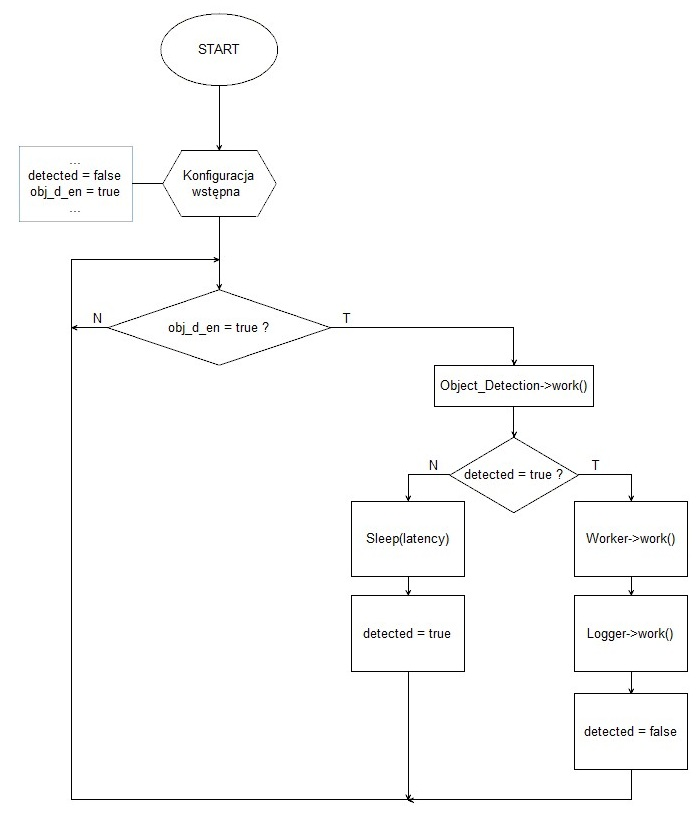
\includegraphics[width=1\linewidth]{sch/algorytm}}
\caption[Algorytm główny aplikacji.]{Algorytm główny aplikacji.}
\label{fig:algorytm}
\end{figure}
\subsection{Aplikacja}
Aby zapewnić elastyczność aplikacji i łatwość rozbudowy oraz debugowania zdecydowano się na modularną strukturę. Wyróżnić można w niej moduł odpowiedzialny za „logikę” – Controller oraz moduły wykonujące zadania – Object Detection, Worker, Logger.
Ważnym aspektem działania aplikacji jest komunikacja między modułami. W projekcie wykorzystano mechanizm sygnałów biblioteki Boost.
\begin{figure}[bth]
\centering
{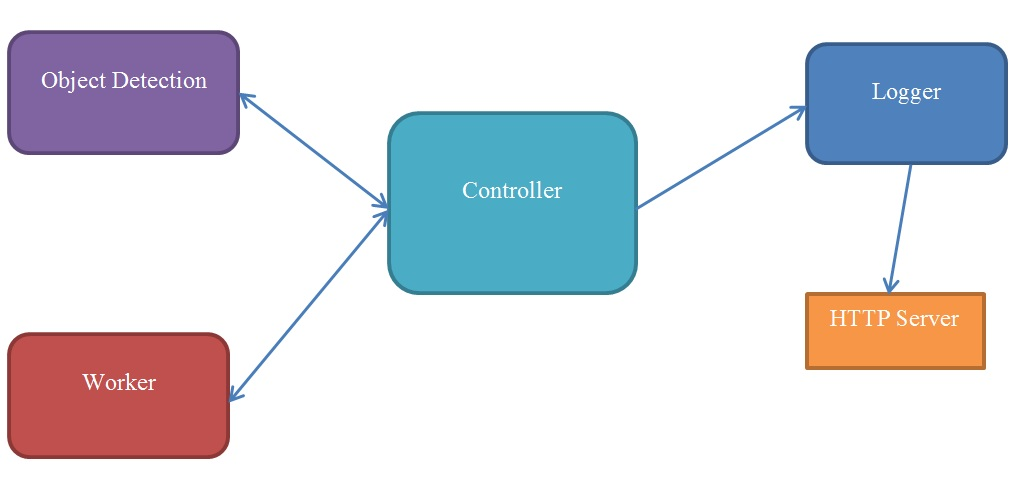
\includegraphics[width=1\linewidth]{sch/kooperacja_obiektow}}
\caption[Diagram współpracy obiektów]{Diagram współpracy obiektów.}
\label{fig:koooperacja}
\end{figure}

\paragraph{Controller} jest odpowiedzialny za przetwarzanie otrzymanych od innych modułów sygnałów i zlecanie im wykonania odpowiednich zadań. Po otrzymaniu sygnału od modułu Object Detect, Controller z wykorzystaniem mechanizmu sygnałów biblioteki Boost zleca modułowi Worker wykonanie akcji, zaś modułowi Logger  przygotowanie pliku logu, który zostanie przetworzony następnie przez serwer HTTP.
Moduł ten odbiera też sygnał zwrotny od Worker’a, potwierdzający wykonanie akcji i pozwala wznowić pracę modułu Object Detect.


\begin{lstlisting}[caption = {Klasa Controller.}, label=Controller, language=C++]
class Controller{
public:
	typedef boost::signals::connection conn;
	short int cam_w,cam_h,latency;
	boost::signal <bool(void *wsk)>SigC;
	bool detected;

	Module * modules[3];
	bool logicUnit(int nr,void* wsk);
		Controller(int w=320,int h=240,int l=2000);
		~Controller();
	
	private:
		conn c_obd;
		conn c_wor;
		conn c_log;
	};     
\end{lstlisting}


\begin{figure}[bth]
\centering
{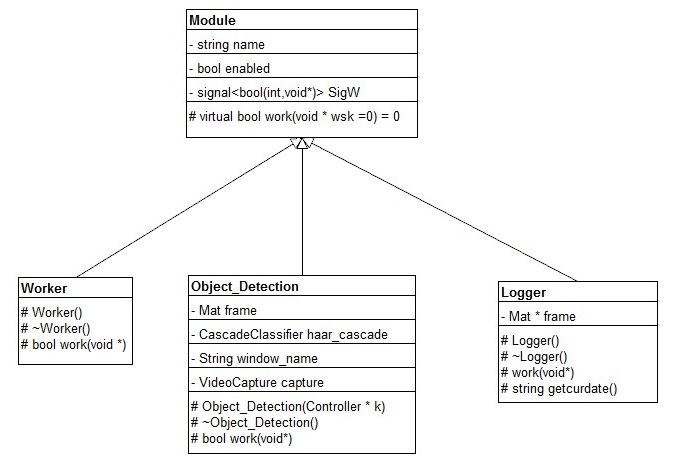
\includegraphics[width=1\linewidth]{sch/diagram_klas}}
\caption[Diagram klas roboczych]{Diagram klas roboczych.}
\label{fig:dziedziczenie}
\end{figure}
Na schemacie \ref{fig:dziedziczenie} zaprezentowana jest implementacja klas roboczych. Wszystkie moduły robocze dziedziczą po abstrakcyjnej klasie Module. Dzięki temu możliwa jest łatwa kontrola i dalsza rozbudowa aplikacji. Implementacja ta jest szczególnie przydatna przy pracy w zespole. Dzięki niej programista wykorzystujący moduł napisany przez innego członka zespołu nie musi znać szczegółowej implementacji - wystarczy, że zna ogólny interfejs i specyfikację modułu (w szczególności argumenty jakie powinien przekazać modułowi).

\paragraph{Object\_Detection} ma za zadanie wykryć obiekty ze strumienia video (dostarczanego przez kamerę podłączoną do płyty. Obiektami założonymi w projekcie są twarze ludzkie, jednak aplikacja jest pod tym względem elastyczna tj. wystarczy wytrenować klasyfikator dowolnego obiektu (narzędzie HaarTraining dostarczone w pakiecie z biblioteką OpenCV) i dołączyć  wygenerowany plik XML. Po wykryciu twarzy wysyłany jest sygnał do Controllera wraz ze wskaźnikiem do struktury frame z wyodrębnionymi twarzami z klatki.

\begin{figure}[bth]
\centering
{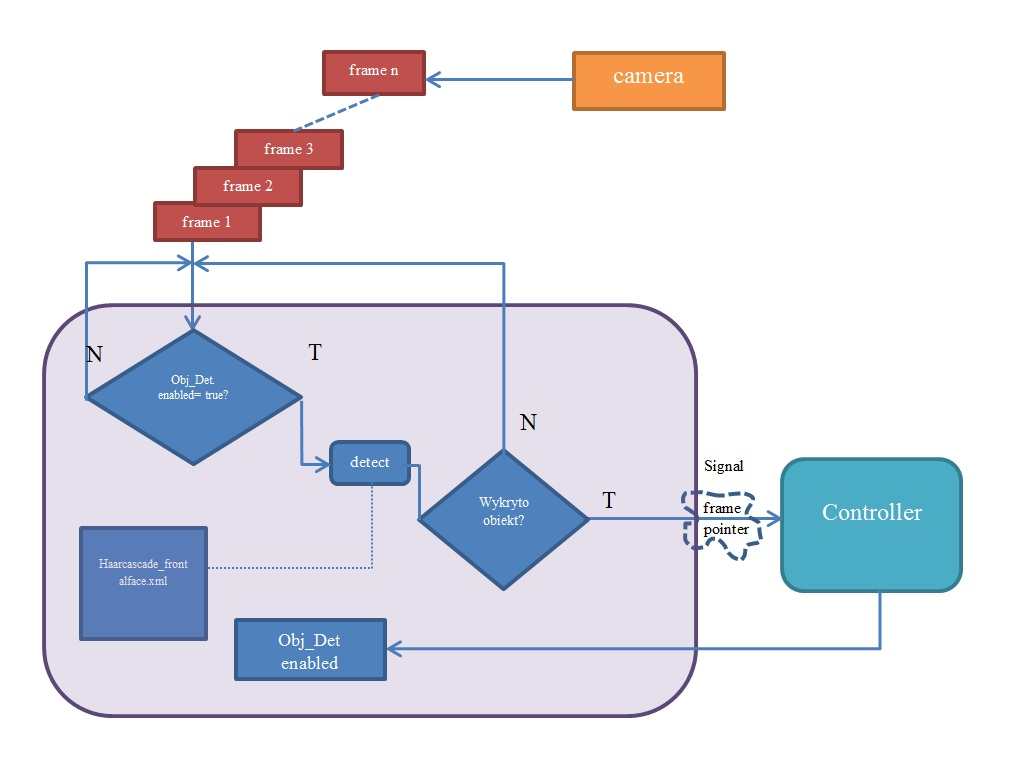
\includegraphics[width=1\linewidth]{sch/detekcja_obj}}
\caption[Schemat działania modułu detekcji obiektów.]{Schemat działania modułu detekcji obiektów .}
\label{fig:detObj}
\end{figure}

\paragraph{Worker} – zadaniem tego modułu jest wykonanie właściwej akcji zadanej przez kamerę. 
W projekcie jest to wystawienie stanu logicznego wysokiego na porcie GPIO, który może przykładowo sterować układem z przekaźnikiem, lub innym układem.
Do implementacji użyto biblioteki wiringPi autorstwa Gordona Hendersona. Biblioteka ta dostarcza łatwy w obsłudze interfejs pozwalający sterować portami GPIO, generować przebiegi PWM, odmierzać czas, oraz wiele innych.
Istotnym zagadnieniem jest mapowanie portów\footnote{Opis mapowania portów znajduje się w dodatku} wirtualnych stosowanych w bibliotece na rzeczywiste wyprowadzenia GPIO.

Na poniższym fragmencie kodu wydruk \ref{Worker} zaprezentowano sposób inicjalizacji biblioteki przez wywołanie funkcji wiringPiSetup(),  a następnie zdefiniowanie portów w konstruktorze klasy Worker.
\paragraph{Logger} - moduł ten odpowiada za wygenerowanie pliku, które skrypty PHP i jQuery po stronie serwera następnie przetwarzają i prezentują użytkownikowi końcowy log. Na listingu \ref{Logger} przedstawiona jest implementacja funkcji roboczej \textbf{work()}.
Moduł rusza do pracy w momencie, gdy obiekt zostanie zdetekowany i zweryfikowany poprawnie.\\
Po otrzymaniu sygnału od \textbf{Controllera} wraz ze wskaźnikiem do struktury \textit{frame} z wykrytym(i) obiektami wywoływana jest robocza funkcja \textbf{work() Loggera}.\\
Kolejnym krokiem jest wyodrębnienie z danej klatki wszystkich twarzy znajdujących się na niej. Do tego wykorzystywany jest wektor \textbf{faces}, w którym to znajdują się współrzędne wszystkich zdetekowanych przez \textbf{Object\_detection} w danej klatce twarzy. W każdej iteracji pętli for tworzona jest oddzielna struktura \textbf{face} typu \textit{Mat} dla każdej twarzy(do tego wykorzystywany jest konstruktor \textit{Mat}, który inicjowany jest klatka \textbf{frame} oraz obszarem zdefiniowanym w wektorze \textbf{faces}, który ma być wyexportowana z \textbf{frame'a}), a następnie generowana jest przez funkcję \textbf{getcurdate()} aktualna data w formacie: [NR\_TWARZY]X[ROK]-[MIESIĄC]-[DZIEŃ]-[GODZINA]:[MINUTA]:[SEKUNDA] , która jest wykorzystana jako nazwa pod, którą zapisywany jest obraz z wyodrębnioną twarzą i rozszerzeniem .jpg. Obrazy zapisywane są w katalogu /var/www/html/faces/. Z tego katalogu skrypt PHP będzie pobierał zdjęcia i przekazywał do skryptu jQuery, aby go następnie przetworzyć i wyświetlić na stronie WWW.
\begin{lstlisting}[caption = {Funkcja robocza klasy Logger.}, label=Logger, language=C++]
extern std::vector<cv::Rect> faces;
bool Logger::work(void* wsk){
	std::cout<<name<<" RUNNING"<<std::endl; 
	std::ofstream log;
	frame = (cv::Mat*)(wsk);
#ifdef TIME_TEST
frame = &test_frame;
#endif
	log.open("/var/www/html/log.txt",std::ios::out | std::ios::app);
	if(!log.is_open())
	  std::cout<<"ERROR READING LOG FILE"<<std::endl;

	for(int i=0; i<faces.size();i++){

		//string index = to_string(i);
	    std::string name = getcurdate()+".jpg";
	    cv::Mat face(*frame,faces[i]);
	    std::string str(name);
	    size_t found= str.find_first_of(":");

	    while (found!=std::string::npos)
	     {
	       str[found]='_';
	       found=str.find_first_of(":",found+1);
	     }

	    log<<name<<std::endl;
	    std::string path;
	    path= "/var/www/html/faces/" + str;
	    printf("%s \n",path.c_str());

	    if( !imwrite(path,face))
	    	std::cout<<"ERROR WRITING IMAGE TO FILE"<<std::endl;
	}

return 0;
}
\end{lstlisting}

\begin{lstlisting}[caption = {Konstruktor klasy Worker.}, label=Worker, language=C++]
Worker::Worker(){

	name="WORKER";
#ifdef BRD_BUILD
	wiringPiSetup();
	pinMode (0,OUTPUT);//GPIO_0 (BCM_GPIO 17) (PHYS. HEADER -> 11)
	pinMode (1,INPUT);	//GPIO_1 (BCM_GPIO 18) (PHYS. HEADER -> 12)
#endif
}
     
\end{lstlisting}

Funkcją odpowiedzialną za akcje wykonywane przez moduł Worker jest work(void * wsk) wyrduk \ref{WorkFun}. Jako argument przyjmuje wskaźnik typu void*, który następnie jest konwertowany do zmiennej int state i dekodowany jest rozkaz od Controllera.

\begin{lstlisting}[caption = {Funkcja work klasy Worker}, label=WorkFun, language=C++]
bool Worker::work(void* wsk){

std::cout<<name<<" RUNNING"<<std::endl;
#ifndef TIME_TEST
int state= *(static_cast<int*>(wsk));
#else
int state = 0;
#endif
	if(state == 0){
#ifdef BRD_BUILD
digitalWrite(0,HIGH);
#endif
std::cout<<"WORKER sets HIGH state"<<std::endl; //open door
#ifndef TIME_TEST
SigW(2,wsk);
#endif
}
else if (state == 2){
#ifdef BRD_BUILD
	digitalWrite(0,LOW);
#endif
	std::cout<<"WORKER sets LOW state"<<std::endl; //close door
#ifndef TIME_TEST
	SigW(2,wsk);
#endif
}
else
{}

	return false;
}

\end{lstlisting}

Po wystawieniu stanu moduł przekazuje sterowanie Controllerowi wysyłając sygnał zwrotny SigW wraz z argumentem w postaci otrzymanego na początku wskaźnika wsk.

\section{Realizacja sprzętowa }
\subsection{Raspberry Pi 2 rev.B}
Raspberry Pi jest w ostatnim czasie jedną z najpopularniejszych platform embedded-systems na świecie. Do jej głównych atutów należą : cena, wydajność, darmowy dostęp do narzędzi i innych zasobów, a przede wszystkim wsparcie techniczne ogromnej społeczności z całego świata. Układ jest wszechstronną bazą umożliwiającą tworzenie projektów zarówno na potrzeby początkujących użytkowników jak i tych bardziej zaawansowanych.\\
Raspberry Pi 2 należy do drugiej generacji układów Raspberry. Jego premiera miała miejsce w lutym 2015 roku. Do kluczowych komponentów urządzenia można zaliczyć min. :
\begin{itemize}[noitemsep]
\item CPU BCM2836 firmy Broadcom quad-core ARM Cortex-A7 taktowany zegarem 900MHz.
\item Pamięć 1GB RAM DDR2
\item Jednostka GPU VideCore IV
\item 4 porty USB
\item 40 pinów GPIO (ang. General Purpose Input-Output)
\item Port Ethernet
\item Interfejs kamery - Camera Serial Interface (CSI)
\item Slot kart microSD
\end{itemize}
Wymiary: 85 x 56 mm
Układ zasilany jest napięciem 5V, przez złącze microUSB.
Według źródła \cite{haydenjames} możliwe jest przetaktowanie rdzeni aż do 1100 MHz w specjalnym trybie force\_turbo, jednak wiąże się to z utratą gwarancji i możliwością niestabilnej pracy oraz uszkodzenia układu.
\subsection{Moduł kamery}
W podrozdziale omówione zostaną dostępne na rynku rozwiązania, które można wykorzystać w projekcie.  Do kryteriów kluczowych w projekcie należy zaliczyć : szybkość kamery, interfejs komunikacji oraz cenę. 

\paragraph{Kamera  z interfejsem USB}

USB (ang. Universal Serial Bus) – uniwersalny sprzętowy interfejs komunikacyjny opracowany przez firmy Microsoft, Intel, Compaq, IBM i DEC. Wykorzystujący magistralę szeregową o prędkościach transmisji danych odpowiednio w standardach :

\begin{itemize}[noitemsep]
\item USB 1.1 do 12Mbit/s (1,5 MB/s)
\item USB 2.0 do 480 Mbit/s (60MB/s)
\item USB 3.0 do 5 Gbit/s (625MB/s)
\end{itemize}

Moduły z interfejsem USB są dosyć popularne zwłaszcza w rozwiązaniach desktopowych, gdzie szybkość przesyłu danych nie jest kluczowa. Świetnie sprawdzają się jako urządzenia dostarczające strumienia wideo dla aplikacji VoIP (ang. Voice over IP). Jako dodatkowy atut można wyróżnić często stosowane wbudowane mikrofony.
Do zestawienia wybrano popularną kamerę  HD Webcam C310 firmy Logitech. Kamera należy do średniej półki cenowej, jej wybrane parametry przedstawiono poniżej.


\begin{table}[hbt!]
%\myfloatalign
\caption[Podstawowe parametry kamery HD Webcam C310]{Podstawowe parametry kamery HD Webcam C310}
\begin{tabularx}{\textwidth}{|l|X|} 
 \hline
Standard transmisji danych &	Full Speed USB 2.0 \\
Rozdzielczość Video &	320x240(QVGA), 640x480(VGA) \\
Maksymalna ilość klatek/s &	30fps@ 352x288(CIF) 15fps@640x480(VGA) \\
Pole widzenia FOV (ang. Field of View) &	50st. \\
Wbudowany mikrofon &	Tak\\
Cena &	ok. 120zł\\
\hline
\end{tabularx}  
\label{tab:compareAnalysers}
\end{table}


\paragraph{ Dedykowany moduł RaspiCam z interfejsem MIPI CSI-2. } MIPI CSI-2 (Mobile Industry Processor Interface Camera Serial Interface) definiuje jednokierunkowy interfejs między modułem kamery, a procesorem. Pozwala na uzyskanie transmisji danych do 4Gbps ( po 1Gbps na linię danych). Moduł wykorzystywany w projekcie posiada 2 linie, co daje łączną przepustowość na poziomie 2Gbps.
Innym rozwiązaniem jest dedykowany dla platformy Raspberry moduł RaspiCam z  sensorem  OV5647 firmy OmniVision. 

Moduł ten wysyła dane za pomocą szyny Camera Serial Interface (CSI-2) do procesora BCM2835. Wykorzystywana jest do tego złącze taśmowe 15-pinowe podłączane do gniazda CSI Camera płyty Raspberry Pi 2. Według danych producenta kamera jest w stanie dostarczyć strumień wideo o rozdzielczości 1920x1080 przy 30 klatkach na sekundę.

\begin{table}[hbt!]
%\myfloatalign
\caption[Podstawowe parametry kamery RaspiCam]{Podstawowe parametry kamery RaspiCam}
\begin{tabularx}{\textwidth}{|l|X|} 
 \hline
Standard transmisji danych &	MIPI CSI-2 \\
Rozdzielczość Video &	1080p,720p,640x480(VGA) \\
Maksymalna ilość klatek/s &	30fps@1080p, 60fps@720p, 90fps@640x480 \\
Pole widzenia FOV (ang. Field of View) & 53.5st. (horizontal) 41.41st (vertical) \\
Wbudowany mikrofon &	Nie \\
Cena: &	85zł \\
\hline
\end{tabularx}  
\label{tab:compareAnalysers}
\end{table}


Tabela 4.2 Podstawowe parametry kamery RaspiCam

Jak widać na korzyść modułu dedykowanego działa nie tylko cena, ale także dużo większa wydajność, wsparcie sprzętowe platformy Raspberry, a przede wszystkim transmisja danych dużo lepsza niż w przypadku kamer z interfejsem USB, co ma wpływ na założoną szybkość kamery. Poniżej znajduje się dokładny opis wybranego modułu RaspiCam.
\begin{description}
\item Sercem modułu jest sensor OV5647 w skład którego wchodzą takie bloki jak :
\begin{itemize}
\item rdzeń sensora optycznego z układami odpowiedzialnymi za przechwycenie obrazu i wstępne przetworzenie go
\item procesor obrazu DPC dokonujący dalszej obróbki
\item interfejs wyjściowy przekształcający dane do odpowiedniego formatu
\end{itemize}
\end{description}
Istotną rolę pełnią bloki generujące sygnały synchronizujące obrazu niezbędne układowi odbierającemu do poprawnego odtworzenia obrazu z danych dostarczonych przez sensor.
Urządzenie komunikuje się z procesorem za pomocą interfejsu SCCB ( ang. Serial Camera Control Bus ). Interfejs ten opiera się na protokole komunikacyjnym I2C (znanym też jako Two Wire Interface) wykorzystującym dwie linie : danych - SDA i zegara – SCL. Urządzenie Master – w tym przypadku procesor BCM2836 wysyła do urządzenia Slave - sensora odpowiednie komunikaty, za pomocą których możliwa jest zmiana jego parametrów.
 

\begin{figure}[bth]
\centering
{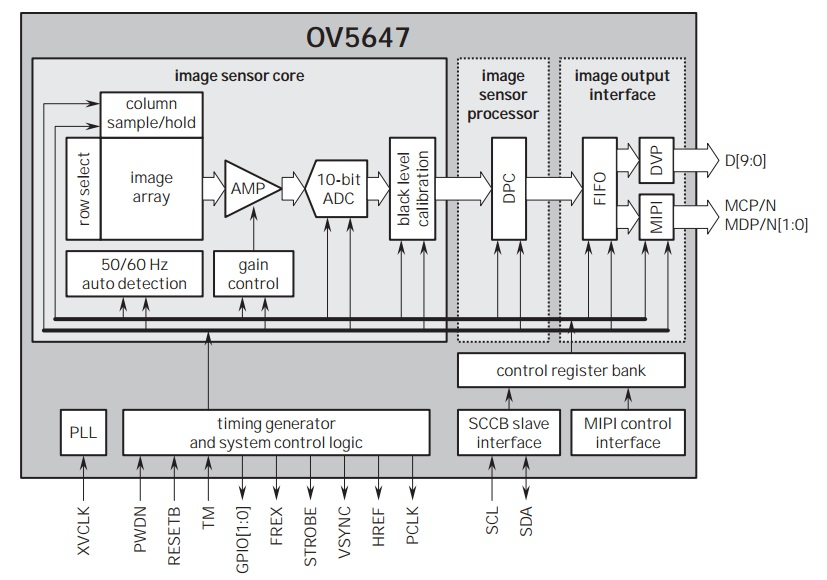
\includegraphics[width=1\linewidth]{sch/OV5647}}
\caption[Schemat funkcjonalny modułu RaspiCam.]{Schemat funkcjonalny modułu RaspiCam.}
\label{fig:detObj}
\end{figure} 

\subsection{Obudowa urządzenia}
Aby zapewnić bezpieczeństwo urządzeniu od wilgoci, zabrudzeń i innych niekorzystnych czynników zastosowana została specjalna obudowa (rys. \ref{}) dedykowana układom Raspberry Pi B+ oraz Raspberry Pi 2. 
Obudowa ta zawiera otwory pozwalające na wyprowadzenie złącz : Ethernet, USB, kamery, wyświetlacza, złącza zasilania - microUSB oraz portów GPIO. Ponadto od wewnętrznej strony zawiera otwory mocowania (za pomocą śrub) modułu RaspiCam oraz otwór na obiektyw kamery, dzięki czemu sensor jest również zabezpieczony.\\
Obudowa została wybrana do celów prototypowych( co nie wyklucza zastosowania jej w rozwiązaniach docelowych). Należy jednak zwrócić uwagę, że po wykonaniu obudowę można zmienić dostosowując jej konstrukcję do wymaganych potrzeb i implementacji. 
